\chapter{Stetigkeit von Abbildungen}
Wir betrachten die Stetigkeit von Abbildungen zwischen metrischen Räumen.
\begin{definition}{Folgenstetigkeit}
	Seien $X$ und $Y$ metrische Räume, wir schreiben für die Metriken von $X$ und $Y$ $\varrho$.
	Die Abbildung $f:X\rightarrow Y$ heißt stetig im Punkt $x_0\in X$, falls aus $x_n\rightarrow x_0$ für eine Folge $(x_n)\in X$ stets folgt:
	\begin{equation*}
		f(x_n)\rightarrow f(x_0)
	\end{equation*}
	Oder kurz, falls gilt:
	\begin{equation*}
		\lim\limits_{n\to\infty}(f(x_n))=\left(\lim\limits_{n\to\infty}f(x_n)\right)
	\end{equation*}
\end{definition}

\begin{multicols}{2}
	\begin{definition}{$\epsilon$-$\delta$-Stetigkeit}
		Seien $X$ und $Y$ metrische Räume.
		Die Abbildung $f:X\rightarrow Y$ heißt stetig im Punkt $x_0\in X$, falls zu jedem $\epsilon>0$ ein $\delta>0$ existiert, so dass gilt:
		\begin{equation*}
			\varrho(f(x),f(x_0))<\epsilon\quad \forall x\in X, \varrho(x,x_0)<\delta
		\end{equation*}
		Oder kurz, falls gilt:
		\begin{equation*}
			f\left(K_\delta(x_0)\right)\subseteq K_\epsilon(x_0)
		\end{equation*}
	\end{definition}

	\columnbreak

	\begin{center}
		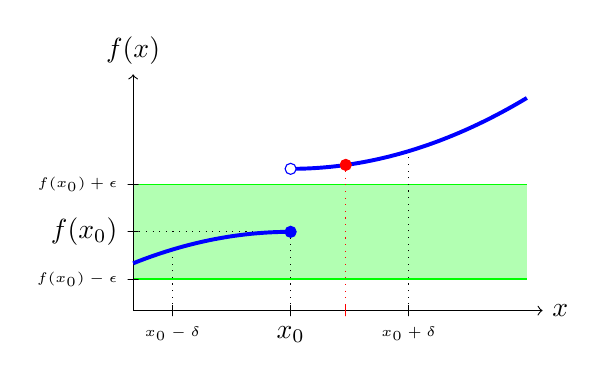
\begin{tikzpicture}
			\fill[fill=green!30!white, draw=none] (0,0.4) rectangle (5,1.6);
			\draw[green, line width=0.2mm] (0,0.4) to (5,0.4);
			\draw[green, line width=0.2mm] (0,1.6) to (5,1.6);

			\draw[->] (0,0) -- (5.2,0) node[right] {$x$};
			\draw[->] (0,0) -- (0,3) node[above] {$f(x)$};


			\draw (2,1) node (fx0) [fill = blue,circle,inner sep = 0pt,minimum size = 4pt,draw = blue] {};



			\draw (2,0) node (x0) [fill = white,rectangle,inner sep = 0pt,minimum size = 0pt,minimum height=4pt,draw, label={below:$x_0$}] {};
			\draw (3.5,0) node (x0pd) [fill = white,rectangle,inner sep = 0pt,minimum size = 0pt,minimum height=4pt,draw, label={below:\tiny$x_0+\delta$}] {};
			\draw (0.5,0) node (x0md) [fill = white,rectangle,inner sep = 0pt,minimum size = 0pt,minimum height=4pt,draw, label={below:\tiny$x_0-\delta$}] {};
			\draw[dotted]
			(x0) -- (fx0)
			(x0md) -- (0.5,0.8)
			(x0pd) -- (3.5,2);




			\draw (0,1) node (fx0achse) [fill = white,rectangle,inner sep = 0pt,minimum size = 0pt,minimum width=4pt,draw, label={left:$f(x_0)$}] {};
			\draw (0,1.6) node [fill = white,rectangle,inner sep = 0pt,minimum size = 0pt,minimum width=4pt,draw, label={left:\tiny$f(x_0)+\epsilon$}] {};
			\draw (0,0.4) node [fill = white,rectangle,inner sep = 0pt,minimum size = 0pt,minimum width=4pt,draw, label={left:\tiny$f(x_0)-\epsilon$}] {};
			\draw[dotted] (fx0achse) -- (fx0);

			\draw[line width=0.5mm, scale=1, domain=0:2, smooth, variable=\x, blue] plot ({\x},{-0.1*(\x-2)*(\x-2)+1}) node[below right] {};

			\draw[line width=0.5mm, scale=1, domain=2:5, smooth, variable=\x, blue] plot ({\x},{0.1*(\x-2)*(\x-2)+1.8}) node[below right] {};
			\draw (2,1.8) node [fill = white,circle,inner sep = 0pt,minimum size = 4pt,draw = blue] {};


			\draw (2.7,1.85) node (fehler) [draw=red, fill=red, minimum size=4pt, circle, inner sep=0pt] {};
			\draw (2.7, 0) node (fehlerachse) [draw=red, minimum size=0pt, minimum height=4pt, inner sep=0pt] {};
			\draw[dotted, red] (fehler) -- (fehlerachse);



		\end{tikzpicture}
	\end{center}
\end{multicols}





\begin{satz}{}
	Folgenstetigkeit und $\epsilon$-$\delta$-Stetigkeit sind äquivalent.
\end{satz}
\beweis
\begin{description}
	\item[\glqq$\Rightarrow$\grqq] Sei $f$ folgenstetig bei $x_0$. Angenommen $f$ wäre nicht $\epsilon$-$\delta$-stetig bei $x_0$:
	Dann gibt es ein $\epsilon>0$ so dass für alle $\delta>0$ ein $x\in K_\delta(x_0)$ existiert, so dass $f(x)\not\in K_\epsilon(f(x))$.
	Wir wählen $\delta=\frac1n$. Dann gibt es zu jedem $n\in\N$ ein $x_n$ mit $f(x_n)\not\in K_\epsilon(f(x_0))$ und $\varrho(x_n,x_0)\to 0$. Widerspruch zur Folgenstetigkeit!
	\item[\glqq$\Leftarrow$\grqq] Es gelte $\epsilon$-$\delta$-Stetigkeit in $x_0$.
	Sei $(x_n)$ eine Folge in $X$ mit $(x_n)\to x_0$.
	Dann gibt es zu jede, $\epsilon>0$ ein $\delta>0$ so dass aus $\varrho(x_n,x_0)<\delta$ folgt, dass $\varrho(f(x_n),f(x_0))<\epsilon$.
	Da $(x_n)\to 0$ konvergiert, gibt es ein $n_0\in\N$ so dass die Folgenglieder $\varrho(x_n,x_0)<\delta$ für alle $n\geq n_0$ gilt, woraus $\varrho(f(x_n),f(x_0))<\epsilon$ folgt, d.h. wir haben $f(x_n)\to f(x_0)$ gezeigt.
	\hfill$\Box$
\end{description}

\begin{definition}{Stetigkeit von Abbildungen}
	Eine Abbildung $f:X\rightarrow Y$ zwischen zwei metrischen Räumen heißt stetig, falls $f$ stetig in allen $x\in X$ ist.
\end{definition}

\paragraph{Bemerkung:}
$f:X\rightarrow Y$ ist stetig genau dann, wenn
\begin{equation*}
	\lim\limits_{n\to\infty}f(x_n)=f(\lim\limits_{n\to\infty}x_n)
\end{equation*}
für alle konvergenten Folgen $(x_n)$ in $X$ gilt.
Stetigkeit bedeutet, dass man Funktionsanwendung und Limes vertauschen kann.

\paragraph{Beispiele:}
\begin{itemize}
	\item Es sei $X=Y=\R$ und $\varrho$ die Standardmetrik in $\R$ für beide.

	Wir betrachten die Abbildung $f:\R\rightarrow\R,x\mapsto x^2$. Wir zeigen jetzt: $f$ ist stetig in allen $x\in X$.

	Dazu betrachten wir eine beliebige Zahlenfolge $(x_n)$ mit $(x_n)\to x_0$ für ein beliebiges $x_0\in\R$.
	Für die Folge der Bildpunkte gilt:
	\begin{equation*}
		|f(x_n)-f(x_0)|=|x_n^2-x_0^2|=|x_n-x_0|*|x_n+x_0|
	\end{equation*}
	Da die Folge $(x_0)$ nach Annahme konvergiert, ist sie beschränkt und es gilt
	\begin{equation*}
		|x_n+x_0|\leq|x_n|+|x_0|\leq M=\mathrm{const.}
	\end{equation*}
	Somit folgt daraus
	\begin{equation*}
		|f(x_n)-f(x_0)|\leq\underbrace{|x_n-x_0|}_{\to 0}*M
	\end{equation*}
	Also folgt $f(x_n)\to f(x_0)$, was die Stetigkeit zeigt.\hfill$\Box$

	\item Sei wieder $X=Y=\R$ und $\varrho$ wie oben.

	Die Funktion $H$ gegeben durch
	\begin{equation*}
		H:X\rightarrow Y, x\mapsto
		\begin{cases}
			0 \text{, falls }x<0\\
			1 \text{ sonst.}
		\end{cases}
	\end{equation*}
	Diese ist unstetig im Punkt $x_0=0$.

	Denn es gilt für die Folge $(x_n)=-\frac 1n$, dass $H(x_n)=H(-\frac 1n)=0\neq H(0)=1$
\end{itemize}

\section{Funktionenlimes, Funktionsgrenzwerte}
Sei $X=Y=\R$ oder $X=Y=\C$ und $\varrho$ der übliche Abstand. Man kann folgende Schreibweise für die Stetigkeit einer Funktion $f:X\rightarrow Y$ im Punkt $x_0$ verwenden:
\begin{align*}
	&f(x_0)=\lim\limits_{x\to x_0}f(x)\\
	:\Longleftrightarrow\enspace&\forall\epsilon>0 \enspace\exists\delta>0 \enspace\forall x\in X:|x-x_0|<\delta \Rightarrow |f(x)-f(x_0)|<\epsilon
\end{align*}
Der Funktionenlimes kann auch für nicht notwendig stetige Funktionen definiert werden, dafür definieren wir rechts- bzw. linksseitigen Grenzwert im reellen Raum wie folgt:
\begin{definition}{Linksseitiger Grenzwert}
	Man schreibt für den linksseitigen Grenzwert
	\begin{align*}
		&\lim\limits_{x\to x_0^-}f(x)=a_l\\
		:\Longleftrightarrow\enspace&\forall\epsilon>0 \enspace\exists\delta>0 \enspace\forall x<x_0:|x-x_0|<\delta \Rightarrow |f(x)-a_l|<\epsilon
	\end{align*}
\end{definition}
\begin{definition}{Rechtsseitiger Grenzwert}
	Und ähnlicch für den rechtsseitigen Grenzwert:
	\begin{align*}
		&\lim\limits_{x\to x_0^+}f(x)=a_r\\
		:\Longleftrightarrow\enspace&\forall\epsilon>0 \enspace\exists\delta>0 \enspace\forall x>x_0:|x-x_0|<\delta \Rightarrow |f(x)-a_r|<\epsilon
	\end{align*}
\end{definition}

\begin{satz}{Stetigkeiten}
	Seien $f$ und $g$ Abbildungen, definiert auf einer Teilmenge von $\R$ oder $\C$.

	$f,g:X\rightarrow Y$ mit $Y=\R$, so dass $f,g$ beide in $x_0\in X$ stetig sind. Dann sind auch folgende Abbildungen stetig:
	\begin{multicols}{2}
		\begin{itemize}
			\item $|f|:x\mapsto |f(x)|$
			\item $c*f:x\mapsto c*f(x)$
			\item $f+g:x\mapsto f(x)+g(x)$
			\item $f*g:x\mapsto f(x)*g(x)$
			\item $\displaystyle\frac{f}{g}:x\mapsto \frac{f(x)}{g(x)}$ mit $g(x)\neq 0$
			\item $\displaystyle\sqrt[p]{f}:x\mapsto \sqrt[p]{f(x)}$ mit $f(x)\geq 0, p\in\N$
			\item $\displaystyle f^p:x\mapsto f(x)^p$ mit $p\in\N$
			\item $f\circ g:x\mapsto f(g(x))$
		\end{itemize}
	\end{multicols}
\end{satz}
\paragraph{Folgerung:}
Reelle oder komplexe Polynome und rationale Funktionen sind in ihrem Definitionsbereich stetig.
\paragraph{Bemerkung:}
Eine Abbildung zwischen metrischen Räumen ist stetig, wenn die Urbilder von offenen Mengen offen sind.
\beweis
\begin{description}
	\item[\glqq$\Rightarrow$\grqq] Sei $V\subseteq Y$ offen, wir müssen zeigen dass
	$U\coloneqq f^{-1}(V) =\set{x\in X}{f(x)\in V}$ offen in $X$ ist.
	Sei dann $x\in U$. Da $V$ offen ist gibt es ein $\delta>0$, so dass $f(K_\delta(x))\subseteq K_\epsilon(f(x))\subseteq V$ ist, was zeigt, dass $K_\delta(x)\subseteq U = f^{-1}(V)$ gilt.

	\item[\glqq$\Leftarrow$\grqq] Sei $x\in X$ und $\epsilon>0$. Dann gilt, dass $U\coloneqq f^{-1}(K_\epsilon(f(x)))$ offen ist, also gibt es zu $x\in U$ ein $\delta>0$, so dass $K_\delta(x)\subseteq U$, woraus $f(K_\delta(x))\subseteq K_\epsilon(f(x))$ folgt.
\end{description}
\paragraph{Bemerkungen:}
Um für Abbildungen zwischen metrischen Räumen Stetigkeit definieren zu können, benötigt man nur die Systeme offener Mengen. Ähnlich kann man Konvergenz von Folgen alleine mit offenen Mengen definieren. Dies führt auf die Topologie. (Stetigkeit und Konvergenz ohne Abstandsbegriff wird auch \glqq Gummigeometrie\grqq\  genannt.)
